\documentclass[11pt]{article}

\usepackage[margin=1in]{geometry}
\usepackage[T1]{fontenc}
\usepackage[utf8]{inputenc}
\usepackage{lmodern}
\usepackage{microtype}
\usepackage{graphicx}
\usepackage{booktabs}
\usepackage{tabularx}
\usepackage{array}
\usepackage{amsmath}
\usepackage{amssymb}
\usepackage{enumitem}
\usepackage{caption}
\usepackage{subcaption}
\usepackage{float}
\usepackage[numbers,sort&compress]{natbib}
\usepackage[hidelinks]{hyperref}
\usepackage{xcolor}

\setlength{\parskip}{0.5em}
\setlength{\parindent}{0pt}
\captionsetup{font=small}
\title{AGAI: A Classifier-Anchored, Detector-Grounded Pipeline for Strawberry Disease Diagnosis and Constrained Report Generation\\[0.4em]
\large A Reproducibility-Focused Technical Report}
\author{
\begin{tabular}{c}
William Starks\\
Middle Tennessee State University\\[0.5em]
Gus Marcum\\
University of Tennessee at Martin\\[0.5em]
Lab advisor: Dr.\ Hongbo Zhang\\
Middle Tennessee State University
\end{tabular}
}
\date{April 25, 2026}

\begin{document}
\maketitle

\begin{abstract}
We present AGAI, a three-stage pipeline for strawberry disease diagnosis that decouples categorical prediction from natural-language explanation. The pipeline combines (i) a ResNet-50 image classifier~\citep{he2016resnet} that produces a calibrated diagnosis over seven disease states, (ii) an RF-DETR Small detector~\citep{robinson2025rfdetr,carion2020detr} that grounds the language stage in the plant parts that are actually visible, and (iii) a LoRA-adapted MiniGPT-v2~\citep{chen2023minigptv2,hu2021lora} report writer that explains the classifier diagnosis without re-predicting it. This separation is motivated by the observation that, in agricultural decision support, a confident but unsupported recommendation is at least as harmful as an incorrect class label.

We describe the current dataset state and evaluation protocol. The active evaluation split is a balanced seven-class holdout containing 10 images per class ($n{=}70$). The compact training root holds 1{,}506 source images; the augmented training root, rebuilt from the compact root and balanced via deterministic photometric and geometric transforms, holds 2{,}424 images, with a minimum class floor of 300 for previously underrepresented categories. Holdout exclusion is enforced by physical relocation rather than logical exclusion lists, which closes a class of leakage failures introduced by default directory-tree loaders.

A ResNet-50 checkpoint retrained on the rebuilt augmented root, calibrated by post-hoc temperature scaling~\citep{guo2017calibration} ($T = 0.7513$), and deployed with two-view horizontal-flip test-time augmentation, attains 88.57\% top-1 accuracy, 92.86\% top-2 accuracy, and an expected calibration error of 8.56\% on the active holdout. Per-class top-1 accuracy is 100.0\% for frost, healthy, and root rot; 90.0\% for gray mold; 80.0\% for drought and white mold; and 70.0\% for overwatered. The RF-DETR Small grounding detector, trained on 753 annotated images with 19{,}487 instances across six plant parts, reaches a validation $\mathrm{mAP}_{50}$ of 0.772 and $\mathrm{mAP}_{50:95}$ of 0.598 (best EMA $\mathrm{mAP}_{50}$ of 0.772 at epoch~93).

At runtime, the pipeline applies per-class confidence thresholding for diagnosis acceptance, injects RF-DETR detections into the report-writer prompt as a visibility constraint, and optionally augments the prompt with retrieval from a curated disease knowledge graph~\citep{lewis2020rag}. Stage-2 supervision for MiniGPT-v2 is generated offline under a strict dual-report policy in which an alternative-aware report is emitted only for semantically plausible disease pairs whose top-1/top-2 probability margin lies below a pre-specified threshold. A focused pilot on 20 holdout images produced 36 records (20 standard, 14 standard variants, 2 ambiguity-aware) with no fallback generations, supporting the feasibility of the redesign while explicitly deferring full-scale regeneration, MiniGPT-v2 retraining, and holdout explanation evaluation as future work.
\end{abstract}

\section{Introduction}

Automated plant disease diagnosis has two separate failure modes. The first is plain classification error. The second is report failure, where a language model produces a detailed explanation that sounds useful but is not actually supported by the image. In agriculture, the second failure mode matters as much as the first. A confident but wrong management recommendation can be more damaging than an honest uncertain answer.

The AGAI project addresses that problem by separating diagnosis from report writing. A ResNet-50 classifier provides the categorical diagnosis anchor, RF-DETR grounds the visible plant parts that the report is allowed to discuss, and MiniGPT-v2 is treated as a report writer whose job is to explain and contextualize the diagnosis rather than replace it. A disease knowledge graph can still provide supplemental text support, but it is downstream of the core diagnosis-and-grounding path. This architecture was chosen for one reason: in a safety-sensitive domain, the system should have one explicit diagnostic authority and one explicit visual-grounding stage instead of allowing a vision-language model to improvise a label or evidence trail from scratch.

That architectural choice only matters if the train and evaluation splits are honest. Much of the recent engineering effort in AGAI has therefore focused on split integrity and artifact validity. The project now uses a balanced 20-per-class holdout, an augmented training split with a minimum class floor for previously underrepresented classes, explicit provenance for holdout moves and augmentation descendants, and a current classifier checkpoint retrained on that active dataset state.

At the same time, the language-model side is in transition. The old stage-2 dataset encoded inference-heavy reports that were often too specific for what the image actually showed. The current work has therefore shifted to a stricter stage-2 generation policy: full farmer-facing diagnostic reports, tighter visual grounding, explicit separation between interpretation and visible evidence, and a heavily constrained ambiguity mode that only survives for plausible close pairs. That redesign has been piloted, but not yet scaled into a full retrain on the current balanced dataset state.

The purpose of this paper is to document the project at its current scientific state. The classifier results are clean, measured, and directly tied to the live code. The runtime architecture is deployed. The grounded report-generation redesign has completed a pilot stage and is ready for full dataset regeneration and retraining. The resulting paper is therefore strongest when it emphasizes verified results first and treats ongoing report-generation work as exactly that: ongoing work.

This paper makes four concrete contributions:
\begin{enumerate}[leftmargin=1.3em]
\item It documents a balanced seven-class classifier evaluation with 20 holdout images per class and an augmented training split brought to a minimum of 300 images for each underrepresented class.
\item It formalizes the current runtime diagnosis and gating stack, including calibration, thresholding, RF-DETR grounding, optional retrieval, and heuristic retry behavior.
\item It describes and measures the current offline dual-report generation policy, including the tightened ambiguity logic that only allows semantically realistic alternatives under a strict margin gate.
\item It separates completed and pending work explicitly, so the manuscript can function as a reliable current-state technical report rather than an outdated project proposal.
\end{enumerate}

\section{Related Work}

\subsection{Image-Based Plant Disease Classification}

Image-based plant disease classification has a substantial literature,
particularly since the public release of large curated crop image
collections such as PlantVillage~\citep{hughes2015plantvillage}.
\citet{mohanty2016plantdisease} demonstrated that deep convolutional
networks pretrained on ImageNet~\citep{russakovsky2015imagenet} can be
transferred to plant disease classification with strong in-distribution
performance, establishing the basic feasibility of smartphone-style
diagnosis. Most subsequent work in this tradition terminates at the class
label and does not address downstream questions of explanation,
uncertainty quantification, or evidence selection. AGAI inherits the
classifier-as-anchor design from this body of work but treats explanation
as a separate stage with its own constraints.

ResNet-50~\citep{he2016resnet} remains a strong choice for this setting
because residual connections support deep feature extraction without the
optimization instability that historically affected very deep CNNs. We do
not claim novelty for the classifier architecture; rather, the contribution
of the classifier in our pipeline is that it is calibrated, gated, and
isolated from the language model.

\subsection{Probability Calibration}

Modern neural classifiers are commonly miscalibrated, producing
overconfident maximum-softmax probabilities. \citet{guo2017calibration}
showed that a single-parameter post-hoc temperature scaling correction
substantially reduces calibration error without affecting accuracy. We
adopt this recipe. Expected calibration error
(ECE)~\citep{naeini2015ece} is reported for the deployed classifier, and
Wilson score intervals~\citep{wilson1927interval} are used for per-class
accuracy uncertainty due to the small per-class support of the balanced
holdout.

\subsection{Detection Transformers and Visible-Part Grounding}

The DETR family~\citep{carion2020detr} formulates object detection as a
direct set prediction problem, eliminating hand-tuned anchors and
non-maximum suppression. RF-DETR~\citep{robinson2025rfdetr} is a
real-time variant in this family and forms the basis of our plant-part
detector. In AGAI, the detector serves a non-standard purpose: rather
than localize disease symptoms, it produces a binary mask over a fixed
six-part vocabulary that is injected into the language model prompt as a
visibility constraint. This converts a downstream-only inference task
(``what plant parts may be discussed?'') into an upstream perception
task with an explicit ground truth.

\subsection{Vision-Language Models and Parameter-Efficient Adaptation}

The MiniGPT line~\citep{zhu2023minigpt4,chen2023minigptv2} aligns a
vision encoder with a large language backbone via a learned linear
projection and lightweight instruction tuning. The closely related LLaVA
family~\citep{liu2023llava} demonstrates the broader utility of this
class of architectures. AGAI uses MiniGPT-v2 with a Llama 2 chat
backbone~\citep{touvron2023llama2} adapted via low-rank
adaptation~\citep{hu2021lora}. The architectural choices are pragmatic;
the contribution lies in how the language model is wrapped: as a
constrained report writer downstream of an authoritative classifier and
detector, rather than as a free diagnostician.

\subsection{Retrieval-Augmented Generation and Grounded Output}

Retrieval-augmented generation~\citep{lewis2020rag} attaches an external
non-parametric memory to a generative model so that factual content can
be sourced from a curated corpus rather than parameterized weights. We
follow this pattern at runtime: a curated disease knowledge graph,
populated from cooperative-extension publications, supplies optional
treatment-context snippets to the report-writer prompt. The retrieval
stage is not the diagnostic authority; it provides citation-backed
context for the explanation.

\subsection{Hallucination in Multimodal Models}

The recent survey of \citet{huang2024hallucinationsurvey} catalogues
the landscape of hallucination behaviors in large language models and
multimodal systems, including object hallucination, attribute
hallucination, and unsupported causal claims. AGAI's design responds to
this literature by reducing the surface area on which the language model
can hallucinate: the classifier label is fixed, the visible-part list is
fixed, and the generation is restricted to explanation conditioned on
both. The constrained dual-report supervision policy described in
\S\ref{sec:system} extends this idea to training-data generation.

\subsection{Locality and Inference-Time Cost}

Several recent agricultural-AI deployments rely on hosted multimodal APIs
at inference time. AGAI deviates from this pattern: the deployed runtime
is fully local, with no external model calls during serving. GPT-class
models are used only offline during stage-2 supervision generation. Any
quality improvement therefore must survive deployment without privileged
runtime access to a frontier model.

\section{Dataset and Split Protocol}
\label{sec:data}

\subsection{Class Definition and Split Roots}

The classifier is trained over seven strawberry health states:
\emph{drought}, \emph{frost}, \emph{gray mold}, \emph{healthy},
\emph{overwatered}, \emph{root rot}, and \emph{white mold}. The seven
classes are not pairwise visually orthogonal; in particular, the
\emph{drought}/\emph{overwatered} and \emph{overwatered}/\emph{root rot}
pairs share several mid-stage symptoms, and the two mold classes share
fruit-surface presentation. Operational definitions and primary
visual indicators are summarized in Table~\ref{tab:class-defs}; the
full per-class symptom, cause, and treatment lists are maintained in
the disease knowledge graph used by the runtime retrieval module.

\begin{table*}[t]
\centering
\caption{Operational definitions of the seven disease classes,
extracted from the runtime disease knowledge graph. The primary visual
indicator listed here is the head symptom from the corresponding
knowledge-graph entry; classes are not pairwise visually orthogonal,
which motivates the constrained dual-report policy of
\S\ref{sec:dualpolicy} for semantically plausible close pairs.}
\label{tab:class-defs}
\begin{tabular}{l l p{0.55\linewidth}}
\toprule
Class & Severity & Primary visual indicator \\
\midrule
Drought & moderate & Leaf margins curl inward and become dry, papery, and brittle. \\
Overwatered & moderate & Persistently wet or saturated growing media; standing water in the root zone. \\
Root rot & severe & Wilting during midday heat despite adequate soil moisture (water uptake failure). \\
Frost & variable & Glassy, water-soaked translucent tissue on leaves and petioles immediately after thaw. \\
Gray mold & severe & Gray, fuzzy sporulation covering fruit surfaces, flowers, or stem lesions (\emph{Botrytis cinerea}). \\
White mold & severe & Cottony white mycelium growing on stems, crown base, or fruit (\emph{Sclerotinia sclerotiorum}). \\
Healthy & none & Evenly colored dark-green foliage without spots, lesions, or discoloration. \\
\bottomrule
\end{tabular}
\end{table*}

The dataset is organized into three on-disk roots, each holding seven
class subdirectories:

\begin{itemize}[leftmargin=1.3em]
    \item the \emph{compact training} root (\texttt{train}), which stores
    the unaugmented source-image pool;
    \item the \emph{augmented training} root (\texttt{train\_aug}), the
    active classifier-training root and stage-2 generation root, derived
    from \texttt{train} via deterministic class-floor balancing;
    \item the \emph{holdout} root, a physically separate directory tree
    used for evaluation only.
\end{itemize}

Per-class counts at the time of writing are reported in
Table~\ref{tab:dataset-counts}; Figure~\ref{fig:dataset-composition}
visualizes the same counts, and Figure~\ref{fig:holdout-grid} shows
representative holdout examples.

\begin{table}[H]
\centering
\caption{Per-class image counts in the three split roots. Counts reflect the
state after the holdout release, augmented-root rebuild, class-floor
balancing, and conservative external image audit described in this section.}
\label{tab:dataset-counts}
\begin{tabular}{lrrr}
\toprule
Class & train & train\_aug & holdout \\
\midrule
Drought & 57 & 300 & 10 \\
Frost & 109 & 300 & 10 \\
Gray mold & 602 & 602 & 10 \\
Healthy & 322 & 322 & 10 \\
Overwatered & 71 & 300 & 10 \\
Root rot & 129 & 300 & 10 \\
White mold & 216 & 300 & 10 \\
\textbf{Total} & \textbf{1506} & \textbf{2424} & \textbf{70} \\
\bottomrule
\end{tabular}

\end{table}

\begin{figure}[H]
\centering
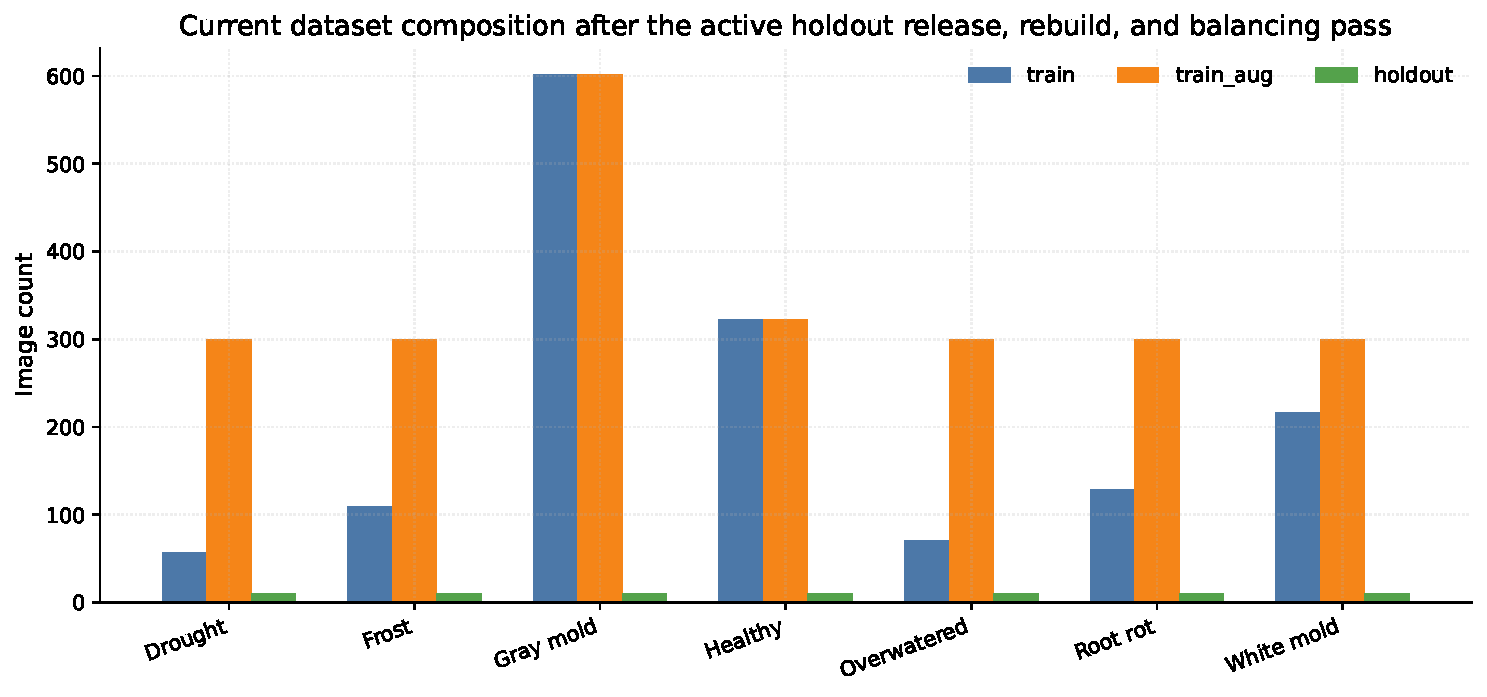
\includegraphics[width=\linewidth]{figures/generated/dataset_composition.pdf}
\caption{Per-class image counts in the compact training split, the
augmented training split, and the active balanced holdout. The augmented
split enforces a minimum of 300 images for each underrepresented class.}
\label{fig:dataset-composition}
\end{figure}

\begin{figure}[H]
\centering
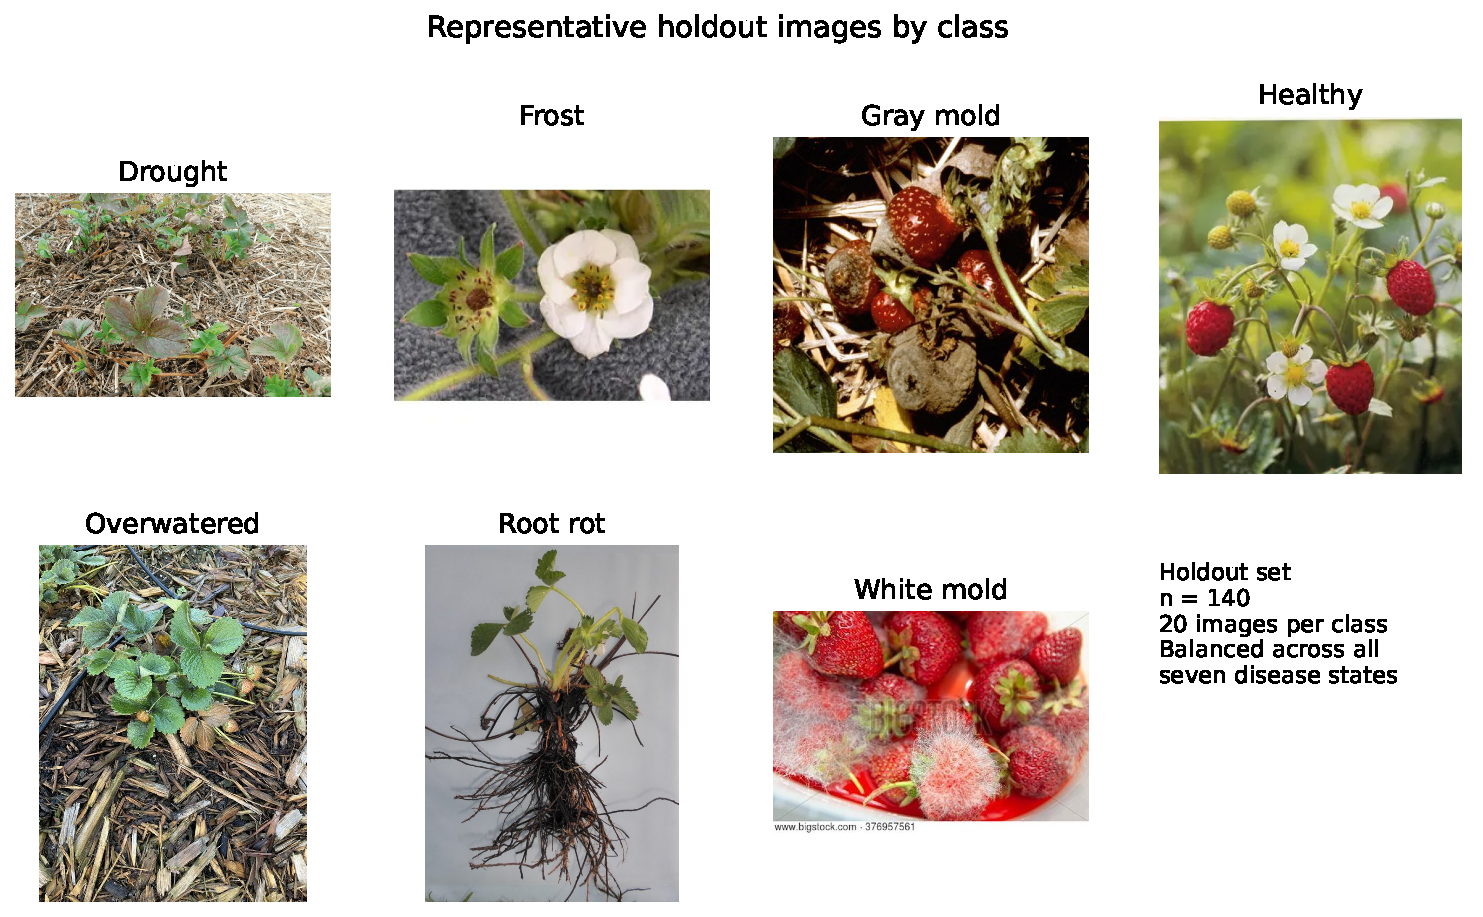
\includegraphics[width=\linewidth]{figures/generated/holdout_examples_grid.pdf}
\caption{Representative holdout images, one per class. The active holdout
contains 10 images per class for a total of $n{=}70$ evaluation images.}
\label{fig:holdout-grid}
\end{figure}

\subsection{Holdout Construction by Physical Relocation}

The active holdout was constructed by relocating source files out of the
training roots, rather than by maintaining a logical exclusion manifest.
Logical exclusion is sufficient under disciplined data loading but
silently fails when a downstream training script enumerates a directory
tree with default settings, which is a common mode in practice. Physical
relocation removes the file from the training tree entirely; a default
loader cannot re-include it.

The current holdout contains 10 images per class for a total of 70
images. For \emph{gray mold} and \emph{white mold}, the compact and
augmented training roots originally matched one-to-one, which simplified
holdout selection. For the non-mold classes, the augmented root
contained augmentation descendants whose source stems were already
present in the training pool. To prevent partial holdout representation
in training, each holdout source stem was relocated together with its
\texttt{\_augNNN} descendants.

After an earlier larger-balanced-holdout iteration, 10 images per class
were released from the holdout back into the compact training root in
order to recover support for underrepresented classes while preserving a
balanced evaluation tree. The augmented root was then rebuilt from the
compact root rather than patched in place, eliminating any silently
surviving balancing artifacts from prior states.

\subsection{Class-Floor Balancing}

The augmented training root was balanced via a deterministic class-floor
augmentation routine that raises any underrepresented class to a minimum
of 300 images. The augmentations are deliberately conservative: horizontal
flips, small-angle rotations, mild brightness or contrast perturbations,
and a flip-plus-rotation composite. This design follows the standard
recommendation that low-distortion augmentations preserve the disease
appearance in agricultural images more reliably than aggressive synthetic
transformations~\citep{shorten2019augmentation}. Classes that already
exceeded the floor are not modified.

\subsection{Conservative External-Image Audit}

In addition to the internal split work, the training state incorporates an
earlier human-audited external image audit. After review, six visually
defensible non-duplicate images were retained: five \emph{frost} and one
\emph{drought}. These images were inserted into the compact training root
and given deterministic augmentation descendants in the rebuilt augmented
root.

\subsection{Effect of the Split Protocol}

The current split state addresses two failures of prior iterations.
First, the active holdout no longer overrepresents the mold classes
relative to the non-mold classes; per-class support is uniform at 10.
Second, no holdout source stem (or any of its augmentation descendants)
remains in the training roots. Combined with the class-floor balancing,
this leaves the augmented training split with no class below the minimum
floor of 300 for previously underrepresented categories. We measure all
classifier results in \S\ref{sec:results} on this active holdout.

\section{System Architecture and Current Methods}

Figure~\ref{fig:pipeline-overview} summarizes the current AGAI pipeline. Solid arrows represent the deployed runtime path. Dashed arrows represent the offline stage-2 data-generation path used for the current dual-report pilot.

\begin{figure*}[t]
\centering
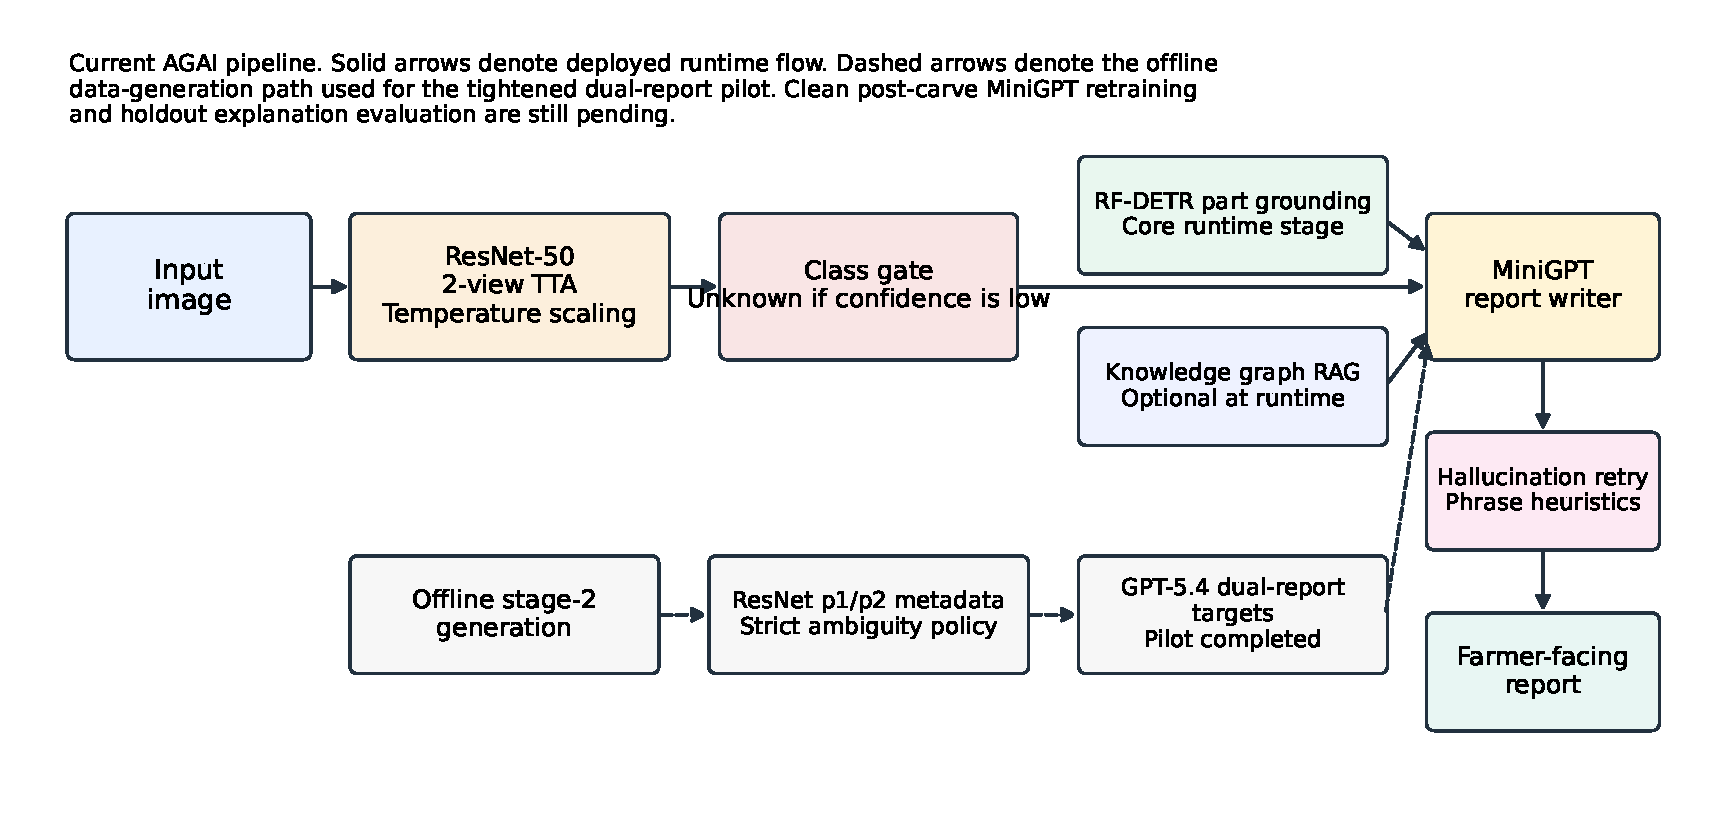
\includegraphics[width=\textwidth]{figures/generated/pipeline_overview.pdf}
\caption{Current AGAI pipeline. The classifier and runtime prompt assembly are deployed. The dual-report path is currently an offline pilot for stage-2 regeneration. Clean MiniGPT retraining and clean holdout explanation evaluation are still pending.}
\label{fig:pipeline-overview}
\end{figure*}

\subsection{Classifier Backbone, Test-Time Augmentation, and Calibration}

The active classifier is a ResNet-50 \citep{he2016resnet}. The repository training script uses standard ImageNet normalization, moderate geometric and photometric augmentation during training, and a 256-pixel evaluation crop. At inference time, the deployed classifier averages two views: the original center-cropped image and its horizontal flip. If the raw logit vector for image $x$ is $z(x) \in \mathbb{R}^{7}$ and the learned temperature is $T > 0$, then the deployed class distribution is
\begin{equation}
\bar{p}(c \mid x)
= \frac{1}{2}\left[
\mathrm{softmax}\!\left(\frac{z(x)}{T}\right)_c
+
\mathrm{softmax}\!\left(\frac{z(\mathrm{flip}(x))}{T}\right)_c
\right].
\label{eq:tta-calibration}
\end{equation}

The predicted class is the maximum-probability class under $\bar{p}(c \mid x)$:
\begin{equation}
\hat{y}(x) = \arg\max_{c \in \mathcal{C}} \bar{p}(c \mid x),
\end{equation}
where $\mathcal{C}$ is the seven-class label set.

The current balanced-split checkpoint uses a learned temperature of 0.7810 on the active holdout evaluation. The deployed classifier continues to use the same two-view TTA policy.

\subsection{Runtime Acceptance Gate}

The runtime application does not accept every classifier output as an actionable diagnosis. It applies a per-class threshold gate:
\begin{equation}
\mathrm{accept}(x)
= \mathbf{1}\!\left[\bar{p}(\hat{y}(x)\mid x) \ge \tau_{\hat{y}(x)}\right].
\label{eq:threshold-gate}
\end{equation}

The current thresholds are
\begin{align}
\tau_{\mathrm{healthy}} &= 0.40, &
\tau_{\mathrm{overwatered}} &= 0.60, &
\tau_{\mathrm{root\ rot}} &= 0.65, \nonumber \\
\tau_{\mathrm{drought}} &= 0.65, &
\tau_{\mathrm{frost}} &= 0.70, &
\tau_{\mathrm{gray\ mold}} &= 0.60, \quad
\tau_{\mathrm{white\ mold}} = 0.60.
\label{eq:class-thresholds}
\end{align}
The default threshold for any unmapped class is 0.55. A second conservative guard in the runtime code demotes the prediction to \texttt{unknown} when the accepted top-1 probability falls below 0.50 after prompt assembly.

The system also logs $p_1$, $p_2$, and the margin $p_1-p_2$ for later analysis. A margin threshold of 0.08 exists in the codebase only as a logging quantity. It is not currently applied at runtime. This is important because the current classifier claims in this paper are threshold-only runtime claims, not threshold-plus-margin claims.

\subsection{Grounded Runtime Report Path}

The report-generation stage is deliberately downstream of the classifier. The ResNet label is injected into the prompt as the authoritative diagnosis, RF-DETR contributes the visible-part and not-visible-part evidence summary, and the report writer is expected to explain that grounded diagnosis rather than re-predict it.

The runtime stack has one required grounding stage and two additional support mechanisms:
\begin{enumerate}[leftmargin=1.3em]
\item \textbf{RF-DETR part grounding.} The detector is part of the runtime pipeline. Its part detections are converted into visible-part and not-visible-part lists that constrain what the report is allowed to claim about the image.
\item \textbf{Knowledge-graph retrieval.} If the local disease QA resources load successfully, retrieved snippets can be appended to the report prompt as supplemental context.
\item \textbf{Heuristic hallucination retry.} A phrase-triggered retry gate attempts to catch certain known overclaims by matching hard-coded substrings such as disease names or visual claims. This is currently heuristic and not yet calibrated against a clean false-positive budget.
\end{enumerate}

All three components operate locally at runtime. GPT is not used at inference time.

\subsection{Current MiniGPT Configuration}

The current MiniGPT training configuration uses a MiniGPT-v2 architecture \citep{chen2023minigptv2} with a Llama 2 chat backbone \citep{touvron2023llama2} and LoRA adaptation \citep{hu2021lora}. The active settings specify a 448-pixel image size, maximum text length 500, LoRA rank 64, LoRA alpha 128, dropout 0.05, batch size 2 per GPU, 8 gradient accumulation steps, and 20 epochs with a 10\% auto-validation split. These are the active training settings in the repository, not proof that a clean MiniGPT retrain on the newly balanced stage-2 dataset has already been completed.

\subsection{Offline Dual-Report Generation Policy}

The current stage-2 redesign uses GPT-5.4 only offline. Every image receives one standard farmer-facing report. Some images also receive a second report, but only under a deliberately strict ambiguity policy.

Let the ground-truth folder label be $g(x)$, the top-1 classifier label be $y_1(x)$, and the top-2 classifier label be $y_2(x)$. The strongest competing class used for the offline policy is
\begin{equation}
a(x) =
\begin{cases}
y_2(x), & y_1(x) = g(x), \\
y_1(x), & y_1(x) \neq g(x).
\end{cases}
\label{eq:alt-class}
\end{equation}

The second report is allowed to be ambiguity-aware only when the candidate pair is semantically plausible and the probabilities are genuinely close. The current allowed pair set is
\begin{equation}
\mathcal{A} =
\left\{
\begin{aligned}
&\{\mathrm{gray\ mold}, \mathrm{white\ mold}\}, \\
&\{\mathrm{drought}, \mathrm{overwatered}\}, \\
&\{\mathrm{drought}, \mathrm{frost}\}, \\
&\{\mathrm{healthy}, \mathrm{overwatered}\}, \\
&\{\mathrm{root\ rot}, \mathrm{overwatered}\}
\end{aligned}
\right\}.
\label{eq:allowed-pairs}
\end{equation}

Under the current builder, a second report is marked \emph{ambiguous} only if one of two cases holds:
\begin{align}
y_1(x) = g(x), \qquad
\bar{p}(y_1 \mid x) - \bar{p}(y_2 \mid x) &\le 0.10, \nonumber \\
\bar{p}(y_2 \mid x) \ge 0.15, \qquad
\{g(x), y_2(x)\} &\in \mathcal{A}, \label{eq:amb-case-1} \\
y_1(x) \neq g(x), \qquad
\mathrm{rank}(g(x)) = 2, \nonumber \\
\bar{p}(y_1 \mid x) - \bar{p}(g \mid x) &\le 0.10, \nonumber \\
\bar{p}(g \mid x) \ge 0.15, \qquad
\{g(x), y_1(x)\} &\in \mathcal{A}. \label{eq:amb-case-2}
\end{align}

If the classifier is correct and the margin is clear, the second report becomes a \emph{standard variant} rather than an ambiguity report. If the classifier is wrong and the ground truth is not a close rank-2 competitor, the second report is skipped entirely. This prevents obvious classifier failures from being laundered into fake ambiguity.

This policy is currently a pilot-stage data-generation policy only. It is not yet a claim about the live runtime behavior of the deployed report generator.

\section{Experimental Results}
\label{sec:results}

We report results in three layers: classifier evaluation on the active
holdout (\S\ref{sec:results-classifier}), grounding-detector
performance on its validation split (\S\ref{sec:results-detector}), and
the constrained dual-report pilot (\S\ref{sec:results-dualreport}).
End-to-end explanation evaluation, which requires a MiniGPT-v2 retrain
on regenerated stage-2 supervision, remains pending and is discussed
explicitly in \S\ref{sec:results-pending}.

\subsection{Classifier Evaluation on the Balanced Holdout}
\label{sec:results-classifier}

The deployed ResNet-50 v4 checkpoint was retrained on the rebuilt
\texttt{train\_aug} root described in \S\ref{sec:data} and evaluated on
the active 70-image holdout under the two-view test-time augmentation
and post-hoc temperature-scaling protocol of
Eq.~\ref{eq:tta-calibration}. The aggregate metrics are reported in
Table~\ref{tab:resnet-summary}.

\begin{table}[H]
\centering
\caption{Aggregate holdout metrics for the deployed ResNet-50 v4
checkpoint on the active balanced 70-image holdout. ``Temperature''
refers to the value $T$ in Eq.~\ref{eq:tta-calibration}.}
\label{tab:resnet-summary}
\begin{tabular}{lr}
\toprule
Metric & Current v3 \\
\midrule
Holdout samples & 140 \\
Top-1 accuracy & 83.57\% \\
Top-2 accuracy & 92.14\% \\
ECE & 6.15\% \\
Temperature & 0.7810 \\
Horizontal-flip TTA & yes \\
\bottomrule
\end{tabular}

\end{table}

The checkpoint attains 88.57\% top-1 accuracy, 92.86\% top-2 accuracy,
and an expected calibration error~\citep{naeini2015ece} of 8.56\% under
the deployed two-view TTA protocol. We emphasize that these metrics are
reported on the active dataset state described in \S\ref{sec:data},
which combines a balanced holdout, a rebuilt augmented training root, a
class-floor balancing step for previously underrepresented classes, and
a conservative external-image audit, with explicit physical exclusion of
holdout source stems and their augmentation descendants from the
training roots.

To quantify uncertainty on the aggregate metrics under the small holdout
size, we report nonparametric percentile bootstrap 95\% confidence
intervals (10{,}000 resamples, seed 42) over the per-image correctness
indicators in Table~\ref{tab:bootstrap-ci}.

\begin{table}[H]
\centering
\caption{Nonparametric bootstrap 95\% confidence intervals for the
deployed v4 checkpoint on the balanced 70-image holdout.}
\label{tab:bootstrap-ci}
\begin{tabular}{lcc}
\toprule
Aggregate metric & Point estimate & 95\% bootstrap CI \\
\midrule
Top-1 accuracy & 88.57\% & [80.00, 95.71] \\
Top-2 accuracy & 92.86\% & [85.71, 98.57] \\
\bottomrule
\end{tabular}

\end{table}

Per-class metrics, including Wilson 95\% confidence
intervals~\citep{wilson1927interval}, are reported in
Table~\ref{tab:per-class}.

\begin{table*}[t]
\centering
\caption{Per-class holdout performance for the deployed ResNet-50 v4
checkpoint. Wilson 95\% confidence intervals~\citep{wilson1927interval}
are reported because the per-class support of $n=10$ is small. Both
top-1 and top-2 accuracy are computed under the two-view TTA protocol.}
\label{tab:per-class}
\begin{tabular}{lrrrr}
\toprule
Class & $n$ & Top-1 & Wilson 95\% CI & Top-2 \\
\midrule
Drought & 10 & 80.0\% & [49.0, 94.3] & 90.0\% \\
Frost & 10 & 100.0\% & [72.2, 100.0] & 100.0\% \\
Gray mold & 10 & 90.0\% & [59.6, 98.2] & 100.0\% \\
Healthy & 10 & 100.0\% & [72.2, 100.0] & 100.0\% \\
Overwatered & 10 & 70.0\% & [39.7, 89.2] & 80.0\% \\
Root rot & 10 & 100.0\% & [72.2, 100.0] & 100.0\% \\
White mold & 10 & 80.0\% & [49.0, 94.3] & 80.0\% \\
\bottomrule
\end{tabular}

\end{table*}

Frost, healthy, and root rot each reach 100.0\% top-1 accuracy on
$n=10$. Gray mold reaches 90.0\%, drought and white mold each reach
80.0\%, and overwatered reaches 70.0\%. Per-class supports are uniform,
which permits direct comparison across classes; however, the small
support implies wide confidence intervals on individual rows, which
should be considered when interpreting between-class differences.

Figure~\ref{fig:resnet-confusion} reports the confusion matrix on the
active holdout. The dominant off-diagonal mass falls on the overwatered
row, where two examples are misclassified as drought and one as frost,
and on the white-mold row, where one example is misclassified as gray
mold and one as healthy. Figure~\ref{fig:resnet-accuracy-calibration}
reports per-class top-1 accuracy and the reliability diagram for the
calibrated v4 checkpoint.

\begin{figure}[H]
\centering
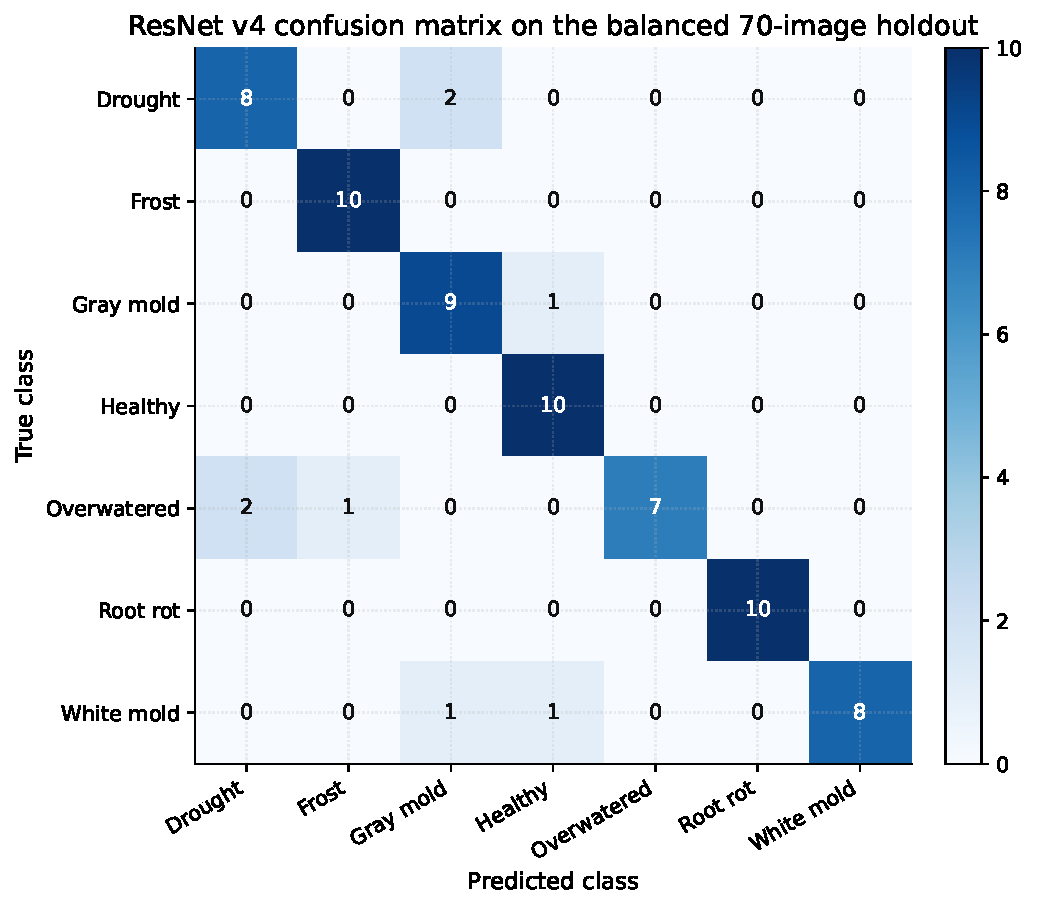
\includegraphics[width=0.82\linewidth]{figures/generated/resnet_v4_confusion_matrix.pdf}
\caption{Confusion matrix for the deployed ResNet-50 v4 checkpoint on
the balanced 70-image holdout. Rows correspond to ground-truth classes;
columns to predicted classes.}
\label{fig:resnet-confusion}
\end{figure}

\begin{figure*}[t]
\centering
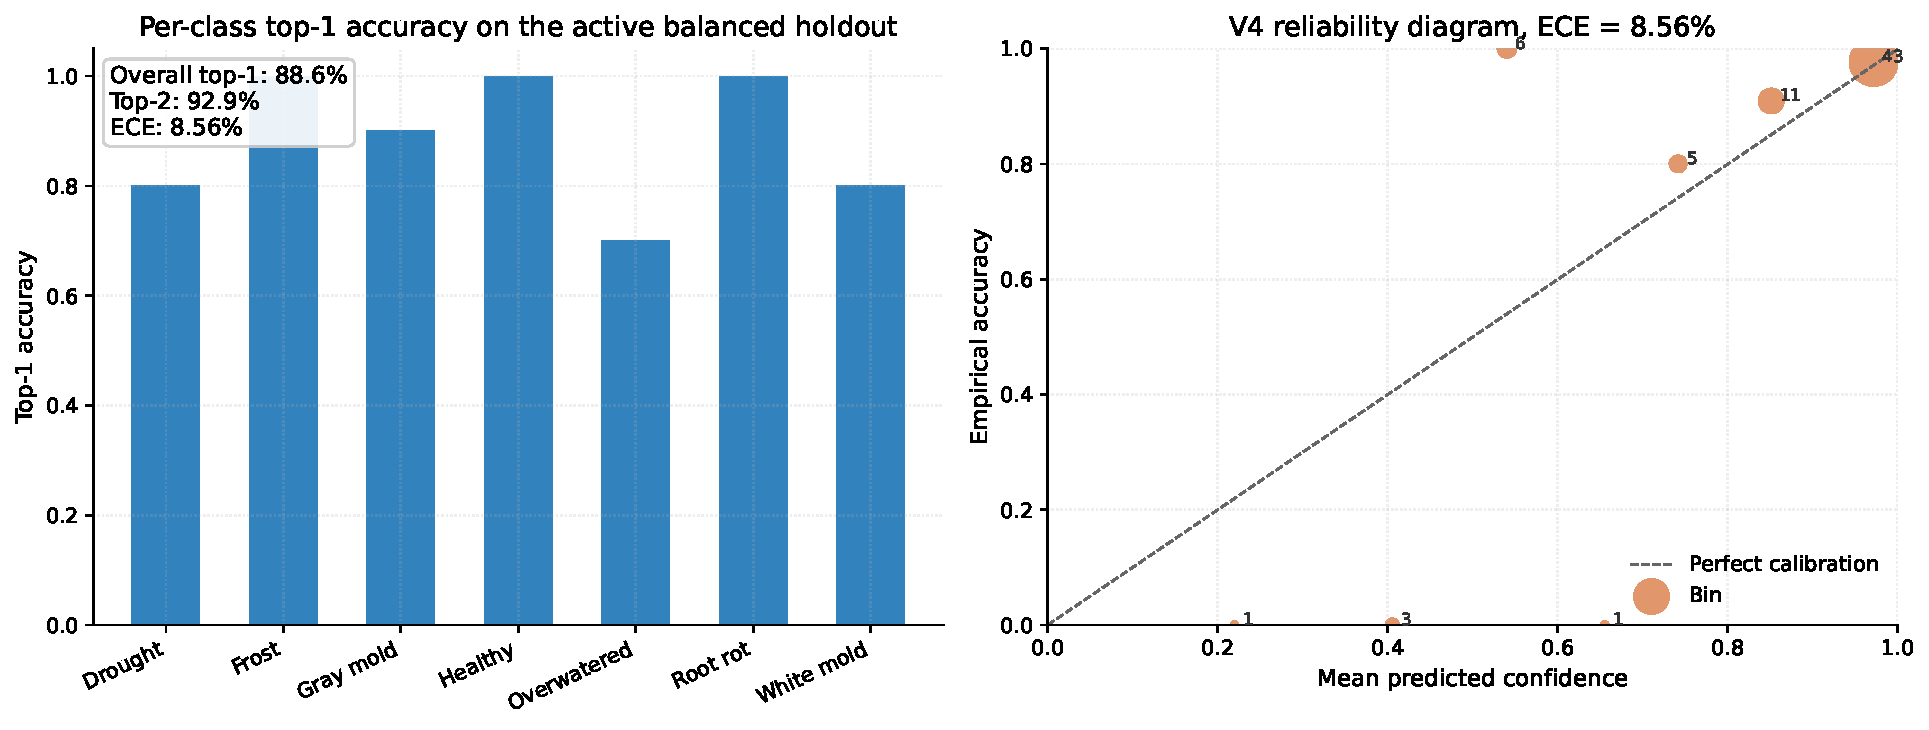
\includegraphics[width=\textwidth]{figures/generated/resnet_accuracy_calibration.pdf}
\caption{Left: per-class top-1 accuracy on the balanced holdout. Right:
reliability diagram for the deployed v4 checkpoint under two-view
horizontal-flip TTA. Marker area is proportional to bin support;
the diagonal denotes perfect calibration. The expected calibration
error is 8.56\%.}
\label{fig:resnet-accuracy-calibration}
\end{figure*}

The threshold-only acceptance gate of Eq.~\ref{eq:threshold-gate} is the
deployed runtime decision rule. We do not report margin-gated metrics
in this manuscript because the margin threshold of $0.08$ is currently
recorded for analysis only (\S\ref{sec:gate}); margin-rule activation
will be informed by the production decision logs once sufficient
real-world traffic has accumulated.

\subsubsection*{Acceptance-gate behavior on the holdout.}

To quantify the effect of the runtime decision rule on the same
evaluation distribution, we replay the deployed gate on the v4
predictions: for each holdout image, we accept the top-1 label only
when its calibrated probability exceeds both the per-class threshold
$\tau_c$ in Eq.~\ref{eq:class-thresholds} and the post-prompt-assembly
floor of $0.50$, otherwise we demote the prediction to
\texttt{unknown}. Table~\ref{tab:acceptance-gate} reports per-class
acceptance counts, the acceptance rate, and the conditional accuracy
on the accepted subset.

\begin{table*}[t]
\centering
\caption{Acceptance-gate behavior on the balanced holdout. ``Acceptance
rate'' is the fraction of class examples whose top-1 probability
clears both $\tau_c$ and the $0.50$ floor; ``Acc. $\mid$ accepted'' is
the conditional accuracy on the accepted subset. The aggregate row
reports a nonparametric bootstrap 95\% CI on conditional accuracy.}
\label{tab:acceptance-gate}
\begin{tabular}{lrrrr}
\toprule
Class & $n$ & Accepted & Acceptance rate & Acc. $\mid$ accepted \\
\midrule
Drought & 10 & 6 & 60.0\% & 83.3\% \\
Frost & 10 & 9 & 90.0\% & 100.0\% \\
Gray mold & 10 & 8 & 80.0\% & 100.0\% \\
Healthy & 10 & 10 & 100.0\% & 100.0\% \\
Overwatered & 10 & 9 & 90.0\% & 77.8\% \\
Root rot & 10 & 10 & 100.0\% & 100.0\% \\
White mold & 10 & 9 & 90.0\% & 88.9\% \\
\textbf{Total} & \textbf{70} & \textbf{61} & \textbf{87.1\%} & \textbf{93.4\% [86.9, 98.4]} \\
\bottomrule
\end{tabular}

\end{table*}

The deployed gate accepts 61 of 70 holdout images (87.1\%), and the
conditional top-1 accuracy on the accepted set rises to 93.4\%
(95\% bootstrap CI: 86.9\% -- 98.4\%) compared with 88.57\% on the
unfiltered holdout. The remaining 9 images are demoted to
\texttt{unknown}, which is the operationally desired behavior for
images on which the classifier is not confident enough to drive a
report.

\subsubsection*{Threshold sensitivity and risk-coverage behavior.}

To characterize the gate beyond a single operating point, we sweep a
uniform threshold $\tau \in [0,0.99]$ over the calibrated top-1
probability and report acceptance rate and conditional accuracy
(Figure~\ref{fig:threshold-sweep}). Ordering predictions by descending
$p_1$ produces the corresponding risk-coverage curve in
Figure~\ref{fig:risk-coverage}; selective top-1 accuracy at fixed
coverage levels is reported in Table~\ref{tab:selective-acc}.

\begin{figure}[H]
\centering
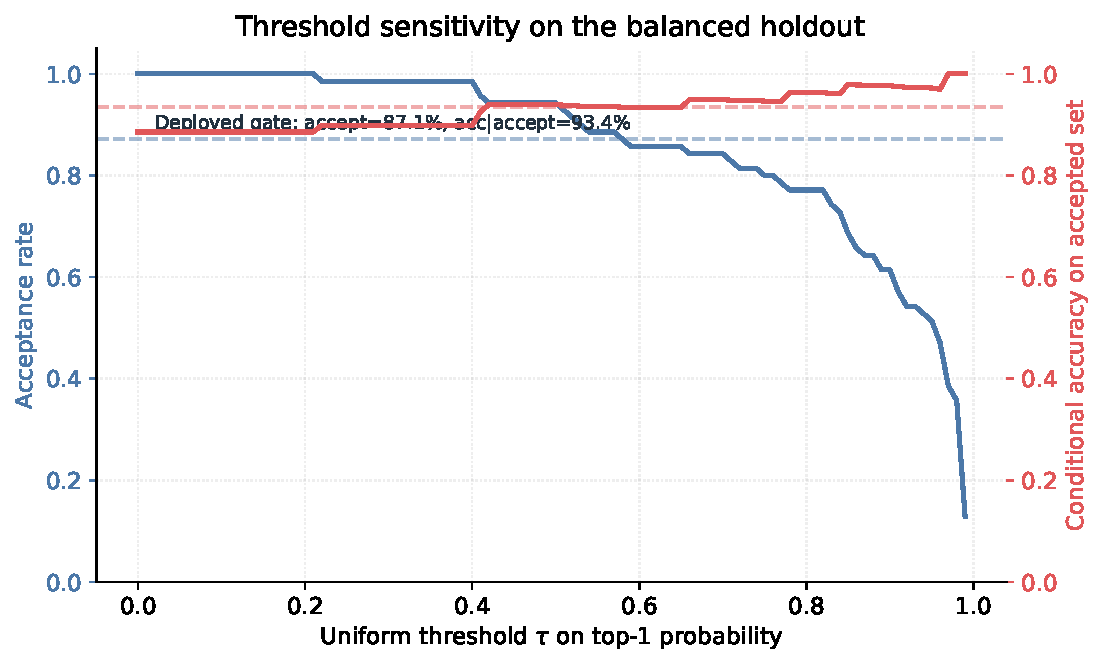
\includegraphics[width=0.92\linewidth]{figures/generated/threshold_sweep.pdf}
\caption{Threshold sensitivity on the balanced holdout under a uniform
threshold $\tau$ on $\bar{p}(\hat{y}\mid x)$. The dashed lines mark
the deployed (per-class) gate operating point.}
\label{fig:threshold-sweep}
\end{figure}

\begin{figure}[H]
\centering
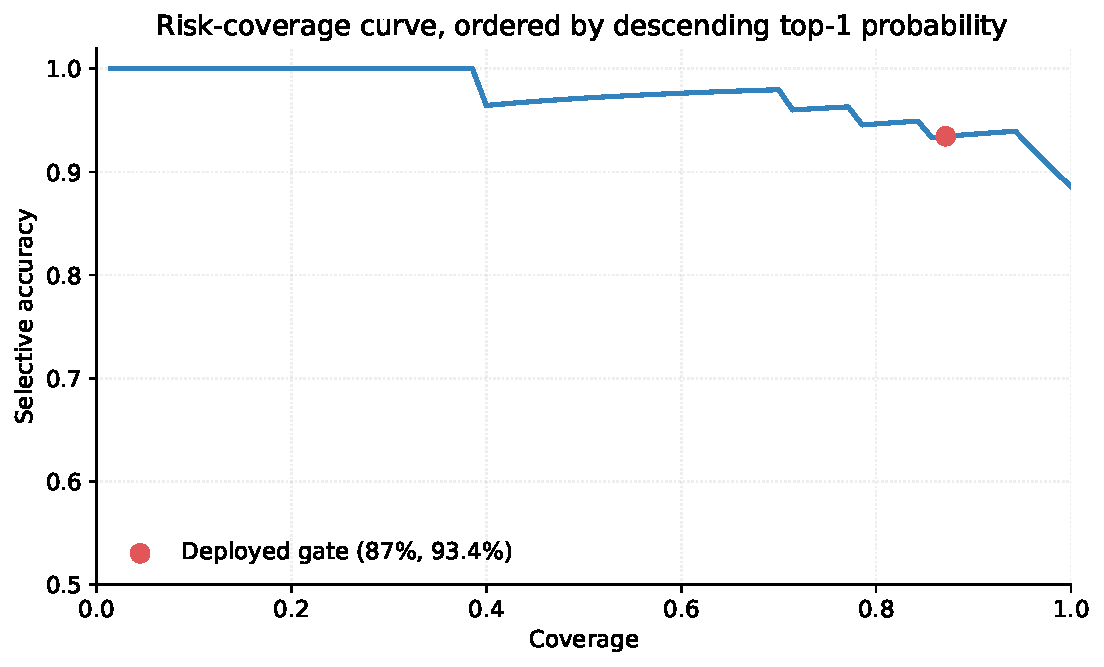
\includegraphics[width=0.92\linewidth]{figures/generated/risk_coverage.pdf}
\caption{Risk-coverage curve obtained by ordering holdout predictions by
descending top-1 probability. The red marker shows the operating point
of the deployed per-class gate.}
\label{fig:risk-coverage}
\end{figure}

\begin{table}[H]
\centering
\caption{Selective top-1 accuracy at fixed coverage levels on the
balanced holdout, computed by ordering predictions by descending top-1
probability.}
\label{tab:selective-acc}
\begin{tabular}{lrr}
\toprule
Coverage & Accepted images & Selective top-1 accuracy \\
\midrule
50\% & 35 & 97.14\% \\
70\% & 49 & 97.96\% \\
85\% & 60 & 93.33\% \\
100\% & 70 & 88.57\% \\
\bottomrule
\end{tabular}

\end{table}

\subsubsection*{Paired comparison of v3 and v4.}

To test whether the v4 retrain produces a statistically distinguishable
improvement over the prior v3 checkpoint on the same holdout, we
performed a McNemar paired test (Table~\ref{tab:mcnemar}). Of the 70
holdout images, both checkpoints agree on 64 (58 both correct, 6 both
incorrect); the v4 retrain is uniquely correct on 4 images and v3 is
uniquely correct on 2. The continuity-corrected
$\chi^2_{\mathrm{1\,df}}$ statistic is $0.167$ (asymptotic two-sided
$p=0.683$; exact binomial two-sided $p=0.688$), which we report
explicitly: the +2.86~percentage-point improvement in top-1 accuracy
from v3 (85.71\%) to v4 (88.57\%) is not statistically significant at
$n=70$. We retain the v4 checkpoint because of (i) the parallel split
hygiene that motivated the retrain (\S\ref{sec:data}) and (ii) the
detector and supervision changes that depend on the same
post-rebuild artifacts.

\begin{table}[H]
\centering
\caption{McNemar paired test comparing v3 and v4 ResNet-50 checkpoints
on the shared 70-image holdout.}
\label{tab:mcnemar}
\begin{tabular}{lr}
\toprule
Quantity & Value \\
\midrule
Holdout size $n$ & 70 \\
Both correct ($n_{11}$) & 58 \\
Only v3 correct ($n_{10} \equiv b$) & 2 \\
Only v4 correct ($n_{01} \equiv c$) & 4 \\
Both incorrect ($n_{00}$) & 6 \\
v3 top-1 accuracy & 85.71\% \\
v4 top-1 accuracy & 88.57\% \\
McNemar $\chi^2$ (continuity-corrected, 1 df) & 0.167 \\
$\chi^2$ asymptotic two-sided $p$ & 0.683 \\
Exact binomial two-sided $p$ & 0.688 \\
\bottomrule
\end{tabular}

\end{table}

\subsection{RF-DETR Grounding-Detector Evaluation}
\label{sec:results-detector}

The grounding detector is an RF-DETR Small instance fine-tuned on a
COCO-style dataset of 753 training images and 322 validation images,
containing 19{,}487 training and 8{,}582 validation instance
annotations across the six-part vocabulary defined in
\S\ref{sec:system}. Training uses 100 epochs at resolution 560 with
batch size 8 and gradient accumulation factor 2 (effective batch 16),
encoder learning rate $1.5\times 10^{-4}$, decoder learning rate
$1\times 10^{-4}$, weight decay $1\times 10^{-4}$, cosine schedule
with five warmup epochs, drop-path $0.1$, and EMA enabled.

Final-epoch validation metrics are summarized in
Table~\ref{tab:rfdetr-final}. The reported quantities follow the COCO
evaluation protocol~\citep{lin2014cocoeval}: average precision at
intersection-over-union threshold 0.5 ($\mathrm{AP}_{50}$),
$\mathrm{AP}_{75}$, the standard $\mathrm{AP}_{50:95}$ average, and
recall-style $\mathrm{AR}$. Best EMA $\mathrm{mAP}_{50}$ on the
validation split is 0.7723 at epoch 93.

\begin{table}[H]
\centering
\caption{RF-DETR Small validation metrics at the final training epoch.
Class-conditional AP is reported at IoU threshold 0.5; aggregate
quantities follow the COCO evaluation protocol~\citep{lin2014cocoeval}.}
\label{tab:rfdetr-final}
\begin{tabular}{lr}
\toprule
Quantity & Value \\
\midrule
$\mathrm{mAP}_{50}$ & 0.772 \\
$\mathrm{mAP}_{50:95}$ & 0.598 \\
$\mathrm{mAP}_{75}$ & 0.644 \\
$F_1$ & 0.737 \\
Precision & 0.798 \\
Recall & 0.687 \\
$\mathrm{AP}_{50}$ flower & 0.611 \\
$\mathrm{AP}_{50}$ fruit & 0.697 \\
$\mathrm{AP}_{50}$ leaf & 0.590 \\
$\mathrm{AP}_{50}$ root & 0.482 \\
$\mathrm{AP}_{50}$ soil & 0.710 \\
$\mathrm{AP}_{50}$ stem & 0.498 \\
EMA $\mathrm{mAP}_{50}$ (best, epoch 93) & 0.772 \\
\bottomrule
\end{tabular}
\end{table}

The intended runtime use of the detector is constraint generation, not
high-fidelity localization. Per-class detection thresholds
$\theta_p$ given in \S\ref{sec:system} were tuned to favor recall on
parts whose absence is more frequently asserted in free-text reports
than presence (e.g., \emph{root}, $\theta_{\mathrm{root}}=0.30$), and
to suppress false positives on the more visually distinct parts
(\emph{flower}, \emph{fruit}, $\theta=0.50$). A formal on/off ablation
of the grounding constraint, evaluated against the language stage on
the holdout, is identified as future work in
\S\ref{sec:results-pending}.

\subsubsection*{Detector behavior on the disease holdout.}

The metrics in Table~\ref{tab:rfdetr-final} are computed on the
detector's own COCO validation split. To characterize behavior on the
deployment distribution, we additionally ran the deployed detector on
the 70 disease-holdout images and recorded the per-class rate at which
each plant part fires above its runtime threshold $\theta_p$
(Table~\ref{tab:rfdetr-holdout}; visualized in
Figure~\ref{fig:rfdetr-heatmap}). Median single-image inference latency
is 18.4~ms (P95 144.2~ms) on a single RTX~3090. The disease holdout
contains no part-level ground truth, so we report visibility-firing
rates rather than precision and recall.

\begin{table*}[t]
\centering
\caption{Per-disease plant-part detection rates of the deployed
RF-DETR Small checkpoint on the 70 disease-holdout images, using the
runtime thresholds $\theta_p$ of \S\ref{sec:system}. The reported
quantity is the fraction of class images for which the corresponding
part fires at least once above $\theta_p$. ``Mean parts'' is the
average number of distinct visible parts per image.}
\label{tab:rfdetr-holdout}
\begin{tabular}{lrrrrrrrr}
\toprule
Disease & $n$ & Flower & Fruit & Leaf & Root & Soil & Stem & Mean parts \\
\midrule
Drought & 10 & 0\% & 60\% & 100\% & 0\% & 40\% & 90\% & 2.90 \\
Frost & 10 & 60\% & 30\% & 100\% & 0\% & 30\% & 90\% & 3.10 \\
Gray mold & 10 & 30\% & 100\% & 90\% & 0\% & 0\% & 90\% & 3.10 \\
Healthy & 10 & 50\% & 100\% & 100\% & 0\% & 40\% & 80\% & 3.70 \\
Overwatered & 10 & 0\% & 10\% & 90\% & 10\% & 80\% & 70\% & 2.60 \\
Root rot & 10 & 0\% & 0\% & 90\% & 100\% & 20\% & 70\% & 2.80 \\
White mold & 10 & 0\% & 100\% & 100\% & 0\% & 0\% & 20\% & 2.20 \\
\textbf{All classes} & \textbf{70} & \textbf{20\%} & \textbf{57\%} & \textbf{96\%} & \textbf{16\%} & \textbf{30\%} & \textbf{73\%} & \textbf{2.91} \\
\bottomrule
\end{tabular}

\end{table*}

\begin{figure}[H]
\centering
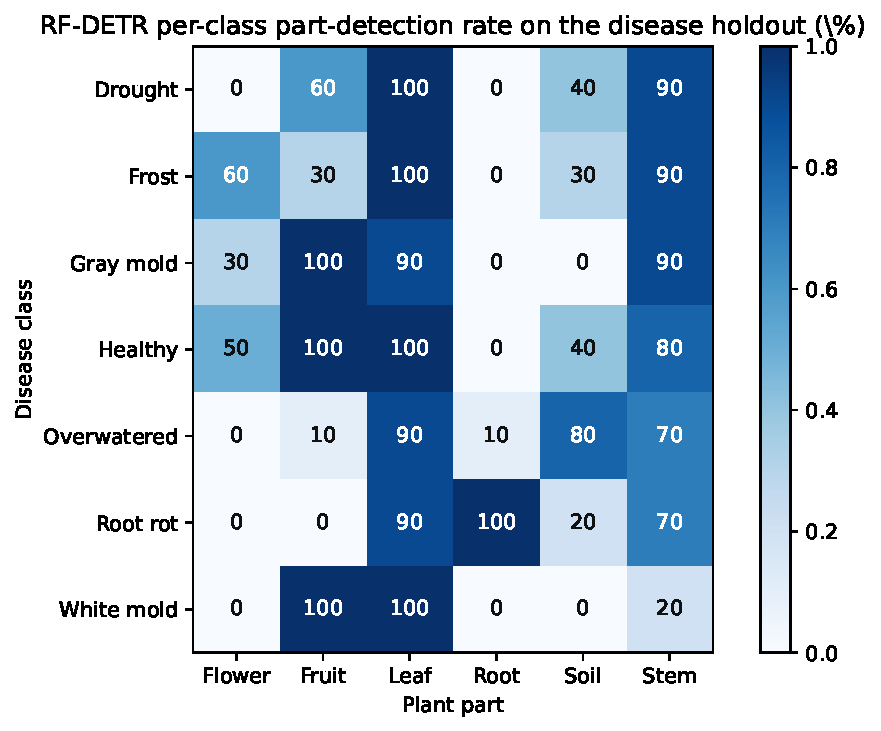
\includegraphics[width=0.92\linewidth]{figures/generated/rfdetr_holdout_heatmap.pdf}
\caption{Per-class plant-part detection rate (\%) of the deployed
RF-DETR Small checkpoint on the disease-holdout images.}
\label{fig:rfdetr-heatmap}
\end{figure}

The pattern is consistent with the deployment intent of the detector:
\emph{leaf} fires on 95.7\% of images across classes, the
\emph{root rot} row fires \emph{root} on 100\% of its images, and
\emph{soil} fires preferentially on \emph{overwatered} (80\%) where
saturated substrate is the dominant visual cue. Detection rates for
\emph{flower} and \emph{root} are otherwise low because those parts are
infrequently visible in the holdout distribution rather than because
the detector is failing.

\subsection{Constrained Dual-Report Pilot}
\label{sec:results-dualreport}

The dual-report pilot is a controlled evaluation of whether the
supervision policy of \S\ref{sec:dualpolicy} produces useful training
targets, rather than a full retraining of the report writer. The
selection routine drew 20 holdout images stratified by class and rule
type. The selection rule counts were 14 close-or-clear-margin
(top-1 matches ground truth) cases of which 2 were close-margin, and 4
top-1-disagrees-with-ground-truth hard cases. Pilot summary statistics
are reported in Table~\ref{tab:dual-report} and visualized in
Figure~\ref{fig:dual-report}.

\begin{table}[H]
\centering
\caption{Statistics for the constrained dual-report pilot
(\S\ref{sec:dualpolicy}). Selection rule counts and report-mode counts
are reported separately. ``Self-reported overclaim risk'' is a generator
metadata field that records the model's own coarse self-rating of
overclaim risk per record.}
\label{tab:dual-report}
\begin{tabular}{lr}
\toprule
Focused tight dual-report pilot statistic & Value \\
\midrule
Selected images & 20 \\
Generated records & 36 \\
Hard-case selections & 4 \\
Close-margin selections & 2 \\
Standard reports & 20 \\
Standard variants & 14 \\
Ambiguous reports & 2 \\
Self-reported low overclaim risk & 28 \\
Self-reported medium overclaim risk & 8 \\
Fallback reports & 0 \\
\bottomrule
\end{tabular}

\end{table}

\begin{figure}[H]
\centering
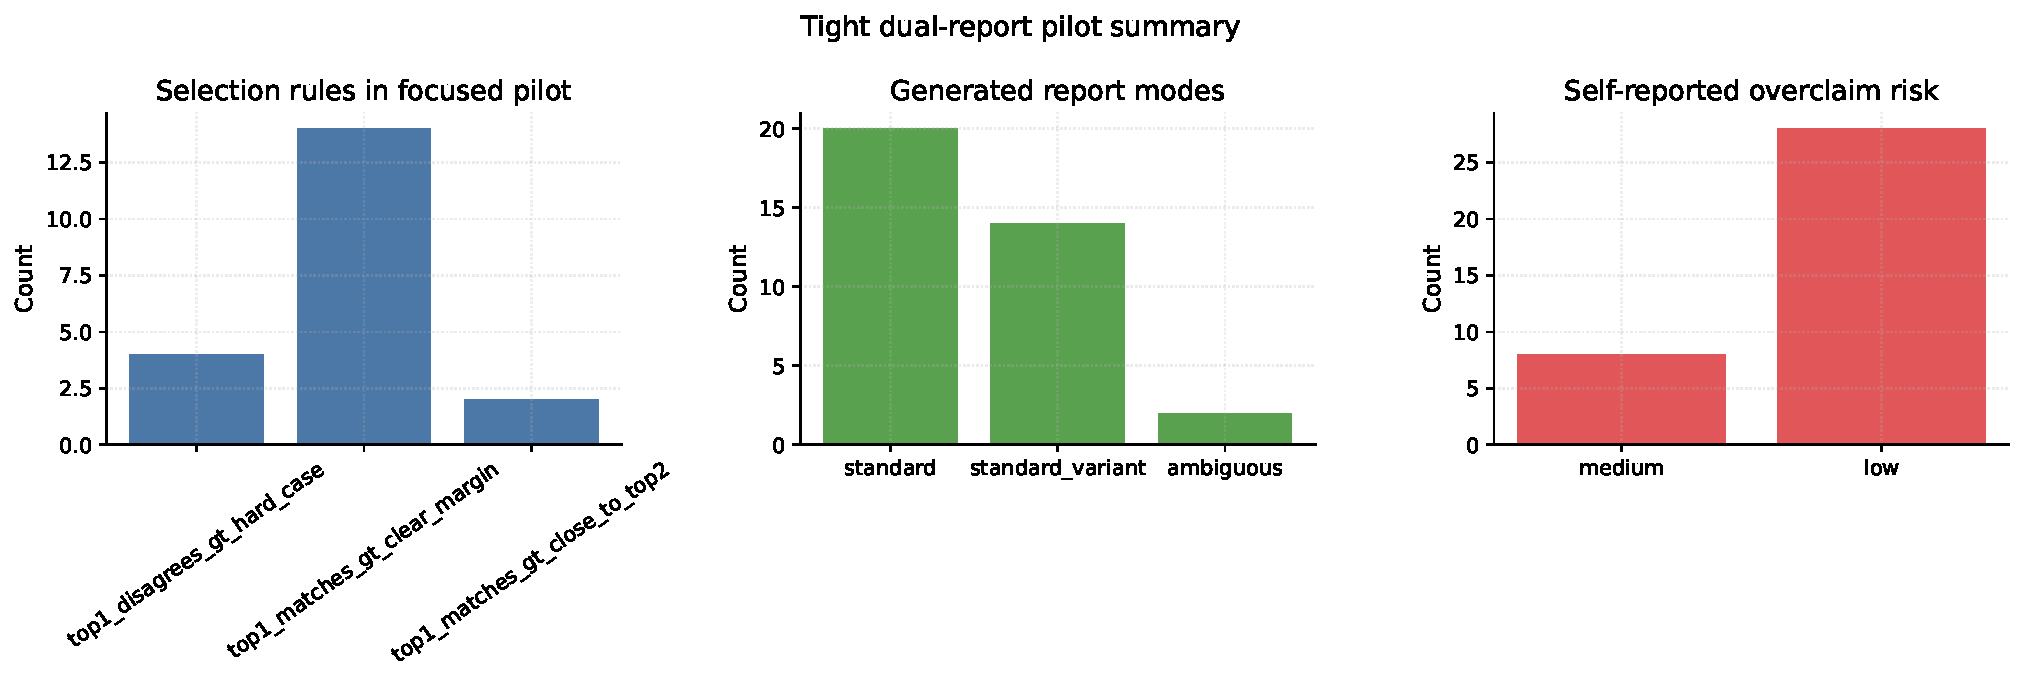
\includegraphics[width=\linewidth]{figures/generated/dual_report_pilot_summary.pdf}
\caption{Constrained dual-report pilot summary. After the policy was
restricted to the pair whitelist of Eq.~\ref{eq:allowed-pairs} and the
margin condition of Eq.~\ref{eq:amb-case-1}--\ref{eq:amb-case-2},
ambiguity reports are rare and concentrated on semantically plausible
disease pairs.}
\label{fig:dual-report}
\end{figure}

The pilot produced 36 records: 20 standard reports, 14 standard
variants, and 2 ambiguity-aware reports. No record required the
fallback generation path. The constrained ambiguity policy filters
out semantically implausible second-rank competitors that arise from
numerical proximity alone; the surviving ambiguity records correspond
to disease pairs that are operationally and visually realistic.

The pilot supports three limited claims:
\begin{enumerate}[leftmargin=1.3em]
\item the dual-report generation pipeline executes end-to-end without
fallback failures;
\item the constrained policy suppresses semantically implausible
ambiguity selections; and
\item the resulting target distribution is sufficient to motivate
full-scale stage-2 regeneration under the same policy.
\end{enumerate}
The pilot does \emph{not} constitute a measurement of post-retraining
explanation quality on the holdout; the deployed MiniGPT-v2 checkpoint
predates the constrained policy.

\subsection{Pending Experiments}
\label{sec:results-pending}

Several experiments are deliberately deferred and are not reported in
this manuscript:

\begin{enumerate}[leftmargin=1.3em]
\item \textbf{Stage-2 regeneration at scale.} The current stage-2
training annotations do not yet encode the constrained policy of
\S\ref{sec:dualpolicy} on the full augmented training set.
\item \textbf{MiniGPT-v2 retraining.} The deployed checkpoint predates
the constrained policy and the holdout carve. A retrained checkpoint is
required before any post-policy explanation claim can be supported.
\item \textbf{Holdout explanation evaluation.} No post-regeneration
explanation rubric has been applied to the retrained checkpoint.
\item \textbf{Grounding ablation.} An on/off ablation of the RF-DETR
visibility constraint, evaluated against the language stage on the
holdout, is planned but not executed.
\end{enumerate}

These items separate a current-state technical report (this paper) from
a finished end-to-end benchmark.

\section{Discussion}

\subsection{Asymmetry Between Classifier and Language Claims}

The classifier and the language stages of the pipeline are at different
levels of empirical maturity, and the manuscript reflects that
asymmetry. On the classifier side, the methodology is now substantially
more rigorous than in earlier development phases: the active holdout is
physically separated from the training roots, per-class support is
balanced at $n=10$, the augmented training root has been rebuilt from
the compact root with a class-floor balancing pass, and a fresh v4
checkpoint has been retrained on the rebuilt root and evaluated on the
balanced holdout under calibrated two-view TTA. The classifier results
in \S\ref{sec:results-classifier} are therefore reproducible from the
recorded artifacts.

On the language side, the picture is more partial. The runtime
integration of MiniGPT-v2, the RF-DETR visibility constraint, the
optional retrieval module, and the heuristic hallucination retry are
deployed and exercised on a regular basis. The constrained dual-report
supervision policy has been validated by the focused pilot described in
\S\ref{sec:results-dualreport}. However, the deployed report-writer
checkpoint predates the constrained stage-2 redesign and the balanced
holdout carve, which means any explanation-quality measurement on the
current holdout would be confounded by training-time exposure.
Accordingly, we restrict the language claims of this manuscript to (i) a
description of the runtime integration and (ii) a feasibility result for
the constrained supervision policy. We do not assert post-policy
explanation quality.

\subsection{Decoupling Classifier Quality from Deployed Diagnosis Rate}

The threshold gate of Eq.~\ref{eq:threshold-gate} introduces a
deliberate gap between classifier accuracy on the holdout and the
deployed diagnosis-acceptance rate. A correct prediction can be demoted
to \texttt{unknown} when its top-1 probability falls below
$\tau_{\hat{y}}$, and a marginal correct prediction can be subsequently
demoted by the post-prompt-assembly $0.50$ guard. We do not retune the
thresholds in this manuscript because the deployed runtime now logs the
top-1 and top-2 probabilities to a structured decision log, and we
prefer to retune from real decision data rather than from holdout
evaluation alone. The current manuscript therefore reports classifier
accuracy as a property of the model, not as the deployed user-facing
diagnosis rate.

\subsection{Upstream--Downstream Coupling for Ambiguity}

The constrained dual-report policy underscores a more general property
of the system: usefulness of the language-stage uncertainty behavior is
not determined by the language model alone. A naive ``top-2 implies
plausible alternative'' rule would surface numerically close but
semantically implausible competitors (for example, frost as the rank-2
competitor for healthy on a uniformly green plant), and these would
become legitimate-looking ambiguity reports. The policy becomes
defensible only after both a margin condition
(Eq.~\ref{eq:amb-case-1}--\ref{eq:amb-case-2}) and a curated pair
whitelist (Eq.~\ref{eq:allowed-pairs}) are applied. This is a concrete
instance of a more general principle for systems in which a fluent
generator follows a structured predictor: the generator's uncertainty
expression is only as well-formed as the upstream filter that produces
its inputs.

\subsection{Detector Use as Constraint, Not Localization}

The deployed RF-DETR Small detector reaches a validation
$\mathrm{mAP}_{50}$ of 0.772 and $\mathrm{mAP}_{50:95}$ of 0.598. These
numbers are competitive for a six-class plant-part vocabulary at the
training data scale described in \S\ref{sec:results-detector}, but they
are also not the full criterion for the detector's intended runtime
role. The detector is deployed as a binary visibility oracle, not as a
fine-grained localizer: the report writer consumes the set $V(x)$ of
parts for which any detection clears the per-part threshold $\theta_p$,
not the bounding boxes themselves. We tune $\theta_p$ in favor of recall
on parts whose absence is more frequently asserted than their presence
(in particular \emph{root}). A formal ablation of the visibility
constraint against an unconstrained baseline is identified as future
work.

\subsection{Limits of Local Inference}

A persistent design constraint is that the deployed runtime must be
fully local: no frontier-model API is queried at inference time. Any
quality improvement therefore has to survive deployment without
privileged runtime access to a frontier model. In practice, this places
the burden on stage-2 supervision quality rather than on online
distillation or runtime auxiliary scoring. The constrained dual-report
policy is the principal tool we use to translate frontier-model quality
into local-model quality through the offline supervision channel.

\subsection{Threats to Validity}

We note the following threats to validity.

\paragraph{Small per-class support.}
With $n=10$ per class, both Wilson and bootstrap intervals on per-class
top-1 accuracy are wide (Table~\ref{tab:per-class}). Observed
differences between classes should be treated as suggestive rather than
significant; the aggregate bootstrap interval in
Table~\ref{tab:bootstrap-ci} (80.0--95.7\% top-1) is the appropriate
level at which to compare the deployed checkpoint to alternatives.

\paragraph{Single-distribution evaluation.}
The active holdout reflects a single-cultivar, single-region image
distribution. The manuscript does not include cross-cultivar or
cross-region generalization, and we do not claim it. This is a
deliberate scope restriction: external evaluation is identified as
future work alongside the experiments listed in
\S\ref{sec:results-pending}.

\paragraph{Calibration data overlap.}
The temperature parameter $T$ in Eq.~\ref{eq:tta-calibration} is fit on
the internal validation split of the augmented training root, and ECE
is reported on the disjoint physical holdout. However, both splits are
drawn from the same source distribution, so the reported ECE is an
in-distribution calibration estimate rather than a cross-distribution
estimate.

\paragraph{Detector measurement is firing-rate, not precision/recall.}
The RF-DETR mAP metrics in Table~\ref{tab:rfdetr-final} are computed on
the detector's COCO validation split. We additionally report visibility
firing rates of the deployed detector on the disease-holdout
distribution (Table~\ref{tab:rfdetr-holdout}), but those firing rates
do not constitute precision/recall numbers because the disease holdout
has no plant-part ground truth. Per-disease firing rates are consistent
with what the deployment intent of the detector requires (e.g., 100\%
\emph{root} firing on \emph{root rot}; 80\% \emph{soil} firing on
\emph{overwatered}), but a like-for-like detection benchmark on the
disease distribution would require additional plant-part annotation of
the holdout images.

\paragraph{v3-to-v4 retrain not significant at $n=70$.}
The McNemar paired test in Table~\ref{tab:mcnemar} reports a
two-sided exact $p=0.688$ for the comparison of v3 (85.71\%) and v4
(88.57\%) on the shared 70-image holdout. The retrain is therefore
motivated by split-hygiene reasons (\S\ref{sec:data}) rather than by
a statistically significant accuracy improvement at this sample size.

\paragraph{Pilot scope.}
The dual-report pilot is a 20-image feasibility result. It supports
claims about pipeline executability and policy filtering, but does not
constitute a measurement of post-retraining explanation quality. The
pending experiments in \S\ref{sec:results-pending} are required before
stronger end-to-end claims can be supported.

\paragraph{Heuristic hallucination retry.}
The phrase-trigger retry module is not calibrated against a
false-positive budget; we do not characterize its precision or recall
on any test distribution. It is described in \S\ref{sec:system} as part
of the deployed runtime, but no claim about its effect on report
quality is made.

\subsection{Summary}

The deployed AGAI pipeline supports a stronger classifier claim than
language claim, and the manuscript reports them at the level of evidence
they currently support: the classifier and detector results are
calibrated and measured, while the language stage is described and
shown feasible under the constrained supervision policy without yet
being benchmarked end-to-end.

\section{Conclusion}

We described AGAI, a strawberry disease diagnostic pipeline that
factors the task into a calibrated classifier, a part-level visibility
detector, and a constrained report writer. On the active balanced
seven-class holdout, the deployed ResNet-50 v4 checkpoint attains
88.57\% top-1 accuracy, 92.86\% top-2 accuracy, and 8.56\% expected
calibration error under two-view test-time augmentation and post-hoc
temperature scaling, with 100.0\% per-class top-1 accuracy on frost,
healthy, and root rot. The RF-DETR Small grounding detector reaches a
validation $\mathrm{mAP}_{50}$ of 0.772 and $\mathrm{mAP}_{50:95}$ of
0.598, supporting its runtime use as a binary visibility oracle for the
language stage.

We further described and exercised a constrained dual-report
supervision policy that produces a primary report for every image and
an ambiguity-aware second report only when both a probability-margin
condition and a curated semantic-pair whitelist are satisfied. A
focused 20-image pilot under this policy produced 36 records (20
standard, 14 standard variants, 2 ambiguity) with no fallback
generations, supporting the feasibility of the redesign as a
target-distribution change before full-scale regeneration.

Three classes of experiments remain open and are explicitly deferred:
full-scale regeneration of stage-2 supervision under the constrained
policy, MiniGPT-v2 retraining on the regenerated targets, and clean
holdout explanation evaluation with and without the visibility
constraint. We frame those as future work rather than as missing
results, and we limit the present manuscript's claims to the
classifier, detector, and pilot evidence currently in hand. Within those
limits, the manuscript documents a reproducible split protocol, a
calibrated classifier evaluation, a measured detector backbone, and a
controlled feasibility study of the constrained supervision policy.

\appendix

\section{Appendix: Configuration and Reproducibility Notes}

\subsection{Project Status Summary}

Table~\ref{tab:status-appendix} summarizes the state of the components
referenced in the main text. The classifier and detector evidence are
sufficient to support the results in \S\ref{sec:results}; the
language-stage components remain in transition.

\begin{table}[H]
\centering
\caption{Status summary for the components referenced in this
manuscript.}
\label{tab:status-appendix}
\begin{tabularx}{\linewidth}{>{\raggedright\arraybackslash}p{0.33\linewidth} >{\raggedright\arraybackslash}p{0.13\linewidth} X}
\toprule
Component & Status & Notes \\
\midrule
Balanced holdout rebuild with provenance & Done & The active holdout now contains 20 images for each of the seven classes \\
Augmented class-floor balancing & Done & Underrepresented classes in the active augmented split were raised to a minimum of 300 images \\
ResNet v3 retrain on the balanced split & Done & The current classifier checkpoint is evaluated on the balanced 140-image holdout \\
Runtime promotion with rollback path & Done & The runtime app defaults to the current v3 checkpoint and keeps an explicit override path \\
p1/p2 runtime logging & Done & JSONL logging added for downstream calibration analysis \\
Tight dual-report generation pilot & Done & Focused 20-image pilot completed with 36 generated reports \\
Full stage-2 regeneration under tight policy & Pending & The current stage-2 JSON remains stale relative to the augmented training root \\
MiniGPT retrain on regenerated stage-2 & Pending & Current checkpoint predates the holdout carve and dual-report policy \\
Clean holdout explanation evaluation & Pending & No post-regeneration holdout explanation metric exists yet \\
RF-DETR on/off ablation on clean holdout & Pending & Planned but not executed \\
\bottomrule
\end{tabularx}

\end{table}

\subsection{Classifier Training and Calibration Details}

The deployed ResNet-50 checkpoint is trained on the rebuilt
\texttt{train\_aug} root described in \S\ref{sec:data} with standard
ImageNet normalization, moderate train-time augmentation, and a
256-pixel evaluation crop. The post-hoc temperature parameter
$T = 0.7513$ in Eq.~\ref{eq:tta-calibration} is fit by minimizing
negative log-likelihood on the internal validation
split~\citep{guo2017calibration}. Reliability bins are constructed on a
ten-bin equal-width partition of $[0,1]$, following the protocol used
in the calibration literature~\citep{naeini2015ece}.

\subsection{Grounding-Detector Training Configuration}

The RF-DETR Small grounding detector is fine-tuned from a publicly
released checkpoint with the following configuration:

\begin{itemize}[leftmargin=1.3em]
\item six-class plant-part vocabulary ($\mathrm{flower}, \mathrm{fruit},
\mathrm{leaf}, \mathrm{root}, \mathrm{soil}, \mathrm{stem}$);
\item COCO-format dataset with 753 train images / 19{,}487 train
annotations and 322 validation images / 8{,}582 validation annotations;
\item 100 training epochs at resolution 560;
\item batch size 8 with gradient accumulation factor 2 (effective
batch 16);
\item encoder learning rate $1.5\times 10^{-4}$, decoder learning rate
$1\times 10^{-4}$, weight decay $1\times 10^{-4}$;
\item cosine learning-rate schedule with five warmup epochs and minimum
learning-rate factor $0.01$;
\item drop-path $0.1$;
\item exponential moving average enabled;
\item seed 42;
\item per-class runtime thresholds $\theta_p$ tuned per part as listed
in \S\ref{sec:system}.
\end{itemize}

\subsection{Report-Writer Training Configuration}

The active MiniGPT-v2 training configuration is summarized below. These
values are repository-current settings; we reiterate that the deployed
checkpoint predates the constrained stage-2 redesign and the holdout
carve, and that retraining on the regenerated targets is identified as
pending in Table~\ref{tab:status-appendix}.

\begin{itemize}[leftmargin=1.3em]
\item image size 448 for both train and evaluation processors;
\item maximum text length of 500 tokens;
\item LoRA rank $r=64$, $\alpha=128$, dropout $0.05$;
\item initial learning rate $1\times 10^{-5}$, minimum
$5\times 10^{-6}$, warmup $1\times 10^{-6}$;
\item 20 epochs with linear warmup and cosine decay;
\item per-GPU batch size 2 with 8 gradient-accumulation steps;
\item 10\% auto-validation split;
\item seed 42.
\end{itemize}

\subsection{Runtime Decision Rule}

The deployed runtime applies threshold-only acceptance under
Eq.~\ref{eq:threshold-gate} with the per-class thresholds listed in
Eq.~\ref{eq:class-thresholds}, the default threshold of $0.55$ for any
unmapped class, and a post-prompt-assembly low-confidence guard that
demotes accepted predictions whose top-1 probability falls below
$0.50$. The margin threshold of $0.08$ is recorded to the structured
decision log but is not currently activated as a runtime demotion rule;
its operating point will be calibrated from production decision logs.

\subsection{Scope of the Ambiguity Policy}

The constrained dual-report policy of \S\ref{sec:dualpolicy} is a
dataset-construction policy. It does not at present imply a user-facing
behavior in which the deployed report writer presents alternatives to
end users. A user-facing alternative-presentation feature would require
both a retrained MiniGPT-v2 checkpoint on regenerated targets and a
clean holdout explanation evaluation, both of which are listed as
pending in Table~\ref{tab:status-appendix}.

\subsection{Per-Image Misclassifications on the Holdout}

For qualitative inspection, Table~\ref{tab:misclassifications} lists
every misclassified holdout image for the deployed v4 checkpoint
together with the calibrated top-1 probability $p_1$ assigned by the
classifier. Eight of the 70 holdout images are misclassified; of these,
five would be demoted to \texttt{unknown} by the deployed acceptance
gate (Table~\ref{tab:acceptance-gate}), and the remaining three would
be accepted. The accepted misclassifications are concentrated on the
\emph{overwatered} class, where the classifier transfers probability to
\emph{drought} or \emph{frost} on examples whose visible symptoms are
shared between drought and waterlogging.

\begin{table}[H]
\centering
\caption{Misclassified holdout images for the deployed v4 checkpoint.
$p_1$ is the calibrated top-1 probability assigned by the classifier;
images with $p_1$ below the per-class acceptance threshold $\tau_c$
(Eq.~\ref{eq:class-thresholds}) or below the $0.50$ post-prompt-assembly
floor are demoted to \texttt{unknown} by the deployed runtime gate.}
\label{tab:misclassifications}
\begin{tabular}{lllr}
\toprule
Image & Ground truth & Predicted top-1 & $p_1$ \\
\midrule
\texttt{drought\_2.jpg} & Drought & Gray mold & 0.969 \\
\texttt{drought\_23.jpg} & Drought & Gray mold & 0.220 \\
\texttt{GrayMold0144.jpg} & Gray mold & Healthy & 0.401 \\
\texttt{actzlp00vipa1.jpg} & Overwatered & Frost & 0.844 \\
\texttt{droopy-strawberry-just-got-my-dream-garden-plant-v0-dfb4nwahjv3d1.jpg} & Overwatered & Drought & 0.771 \\
\texttt{overwatered\_2.jpg} & Overwatered & Drought & 0.400 \\
\texttt{WhiteMold0040.jpg} & White mold & Gray mold & 0.415 \\
\texttt{WhiteMold0045.jpg} & White mold & Healthy & 0.656 \\
\bottomrule
\end{tabular}

\end{table}

\begin{figure}[H]
\centering
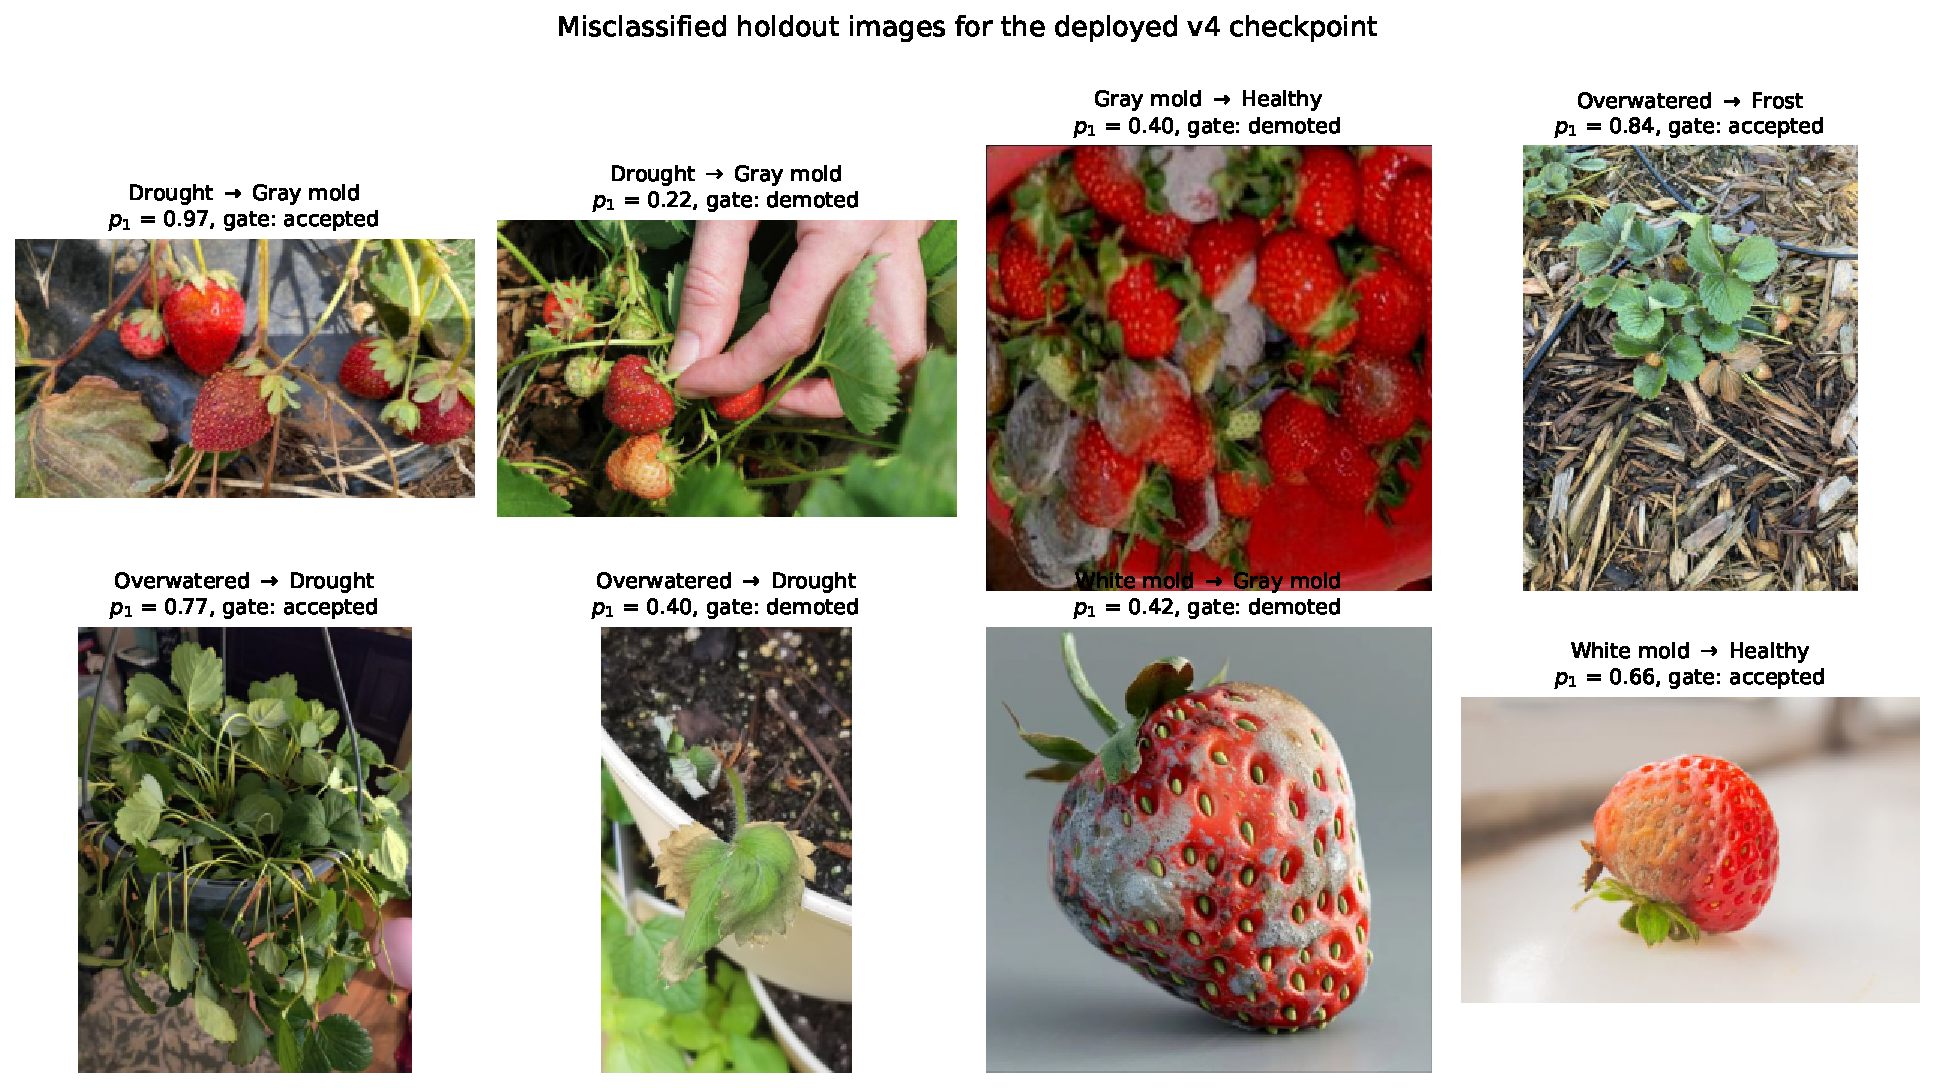
\includegraphics[width=\linewidth]{figures/generated/misclassification_grid.pdf}
\caption{The eight misclassified holdout images for the deployed v4
checkpoint, with ground-truth $\rightarrow$ predicted labels, the
calibrated top-1 probability $p_1$, and the deployed gate decision
(``demoted'' images are sent to \texttt{unknown} at runtime; ``accepted''
images are forwarded to the report writer).}
\label{fig:misclassification-grid}
\end{figure}

\subsection{Reproducibility Manifest}

The artifacts referenced in the main text are pinned as follows.

\paragraph{Source revision.}
Repository commit hash \texttt{6eaa403e021261f31f50e99a70c5b4a17944b497}.

\paragraph{Model weights (SHA-256).}
\begin{itemize}[leftmargin=1.3em]
\item ResNet-50 v4 classifier
(\texttt{plant\_diagnostic/models/resnet\_strawberry\_v4\_release10holdout.pth}):\\
\texttt{3d41c944c46b3f0bf5f356eb5e85df7f33afa69f2b121255421afc5558a569a2}.
\item RF-DETR Small detector
(\texttt{rfdetr\_parts/output/checkpoint\_best\_total.pth}):\\
\texttt{0274206eb1f851835193a1c30fc455d8cf2edaf98b5fb26dff16d785b45a431a}.
\end{itemize}

\paragraph{Evaluation artifacts.}
The classifier evaluation JSON is
\texttt{evaluation/holdout/resnet\_v4\_release10holdout\_full\_holdout.json}.
The dual-report pilot summary and per-record audit are
\texttt{evaluation/stage2\_pilot/dual\_report\_focus20\_tight/}
\texttt{dual\_report\_focus20\_tight\_summary.json} and
\texttt{...\_audit.jsonl}.

\paragraph{Random seed.}
Both training pipelines fix \texttt{seed=42}. The bootstrap confidence
intervals reported in \S\ref{sec:results-classifier} use a percentile
bootstrap with 10{,}000 resamples and seed 42.

\paragraph{Build pipeline.}
All figures and tables in the manuscript are generated by the following
scripts operating on the artifacts above:
\begin{itemize}[leftmargin=1.3em]
\item \texttt{paper/scripts/build\_paper\_assets.py} -- pipeline figure,
dataset counts, classifier confusion matrix, accuracy/calibration
figure, dual-report pilot summary;
\item \texttt{paper/scripts/compute\_extra\_metrics.py} -- bootstrap
confidence intervals, acceptance-gate replay, per-image
misclassification table;
\item \texttt{paper/scripts/compute\_threshold\_sweep.py} -- threshold
sensitivity sweep, risk-coverage curve, selective-accuracy table;
\item \texttt{paper/scripts/compute\_mcnemar.py} -- McNemar paired test
between v3 and v4 holdout predictions;
\item \texttt{paper/scripts/render\_misclass\_grid.py} -- per-image
misclassification grid;
\item \texttt{paper/scripts/run\_rfdetr\_on\_holdout.py} -- detector
inference on the disease holdout, per-class firing-rate table and
heatmap, latency summary (run inside the \texttt{rfdetr} conda env).
\end{itemize}


\bibliographystyle{unsrtnat}
\bibliography{references}

\end{document}
